\section{Les choses se GATT}
\begin{frame}
	\frametitle{ATT}
	\begin{quote}A protocol for discovering, reading, and writing attributes on a peer device.\end{quote}

	\begin{block}{\textbf{ATT}ribute}
		\begin{itemize}
			\item Type : Ce que l'attribut représente (UUID)
			\item Handle : Indentifie l'attribut sur un serveur
			\item Permissions :
				\begin{itemize}
					\item Lecture / Écriture
					\item Notification
					\item Encryption
					\item Autorisation
					\item Authentification
				\end{itemize}
		\end{itemize}
	\end{block}
	Un Attribut est une métadonnée définissant une valeur.
\end{frame}

\begin{frame}
	\frametitle{GATT par l'exemple}
	\center{\textbf{G}eneric \textbf{ATT}ribute Profile}
	\begin{figure}
		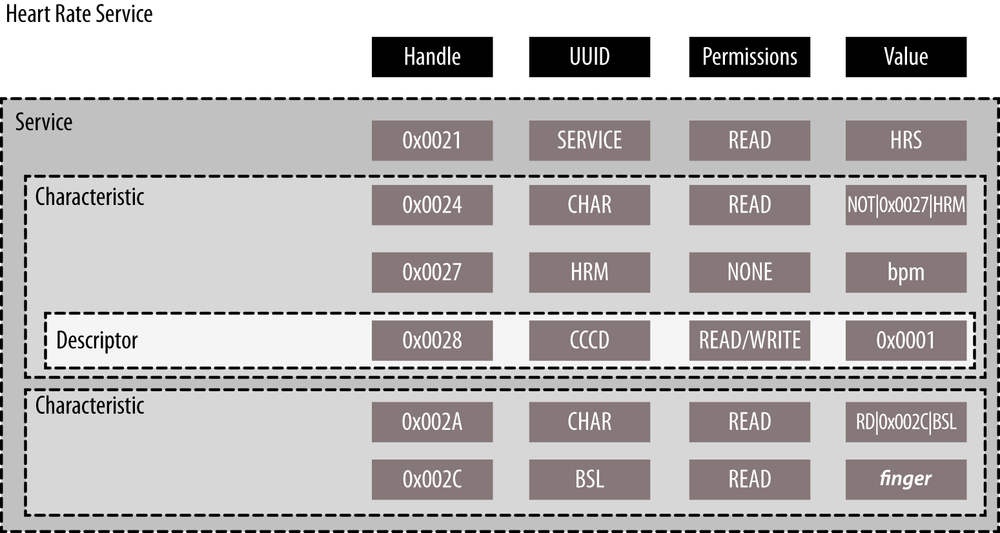
\includegraphics[height=5cm]{img/gatt.png}
	\end{figure}
{\tiny "Getting started with bluetooth low energy", R.Davidson, Akiba, Carles Cufí, Kevin Townsend, O'Reilly}

\end{frame}

